\testCom
{%Номер задачи
	3.17
}
{%Условие
	Два математических маятника, каждый длины l = 50 см и массы m = 45г, соединены пружинкой жесткостью x = 0.66 Н/м. При равновесии маятники занимают вертикальное положение. Найти период малых колебаний этих маятников, если их колебания происходят в вертикальной плоскости в противоположные стороны.
}
{%Дано
	l = 50 см\\
	m = 45г\\
	x = 0.66 Н/м\\
}
{%Найти
	T - ?
}
{%Решение
	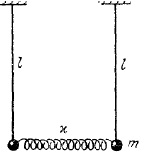
\includegraphics[height=30mm]{3_17.jpg}\\
	$m \frac{dx}{dt^2} = - m g \sin \alpha + \kappa \delta x$\\
	${x}_{1} = 1 - {x}_{2}$\\
	$\delta x = - {x}_{1} - (1 - {x}_{2})$\\
	$m\frac{d^2x}{dt^2}= -mg\sin \alpha - 2 \kappa {x}_{1} \approx - mg \frac{{x}_{1}}{l} - 2\kappa {x}_{1} $\\
	$\frac{d^2{x}_{1}}{dt^2} \approx - (\sqrt{\frac{g}{1} - \frac{2 \kappa}{m}})^2 {x}_{1} = - \omega ^2 x$\\
	$\omega = \sqrt{\frac{mg - 2 \kappa l}{ml}}$\\
	$T=\frac{2 \pi}{\omega} = \frac{2\pi \sqrt{ml}}{\sqrt{mg - 2 \kappa l}}$\
}


